\documentclass[output=paper,newtxmath,modfonts,nonflat,draftmode]{langsci/langscibook} 
\ChapterDOI{10.5281/zenodo.3520595}
\author{Ponsiano Sawaka Kanijo\affiliation{University of Gothenburg}} 
\title{}

\markuptitle{The interaction of \textit{‑ø‑\ldots‑íle}  with aspectual classes in Nyamwezi}{The interaction of ‑ø‑\ldots‑íle  with aspectual classes in Nyamwezi}
\renewcommand{\lsCollectionPaperFooterTitle}{The interaction of \noexpand\textit{‑ø‑\ldots‑íle} with aspectual classes in Nyamwezi}
 
\abstract{This study investigates different readings of the construction -\textit{ø}-\ldots-\textit{íle} resulting from the interaction with aspectual classes in Nyamwezi, a Bantu language spoken in Tabora, Tanzania. The study is motivated by two observations. Firstly, in previous analyses \citep{Maganga1992}, it was noted that -\textit{ø}-\ldots-\textit{íle} in Nyamwezi selects few verbs, but the patterns governing its distribution were not identified. Secondly, not much has been done on describing the semantics of verbal roots in Nyamwezi (and many other Bantu languages), which appears to be a source of variable temporal interpretations of -\textit{ø}-\ldots-\textit{íle}. Based on field data, I show that the first main function of -\textit{ø}-\ldots-\textit{íle} is that of stativizer. That is, -\textit{ø}-\ldots-\textit{íle} picks out a phase of an event or the entire event (if the event lacks phasic structure) and presents it as a stable, undifferentiated property. -\textit{ø}-\ldots-\textit{íle} does so in three different ways, which give three different readings: (i) resultative, when it occurs with achievements, (ii) general present, which occurs with statives and (iii) a progressive-like reading, which occurs with some activity verbs classified as ``directed motion verbs'' in this study. The discussion of the contrast between these readings is informed by a progressive form -{\textit{l}}{\textit{ɪɪ}}-. Many other activity verbs do not typically occur with -\textit{ø}-\ldots-\textit{íle}. Those that occur with this construction either suggest the change-of-state or condition of the verb’s subject (which has the semantic role of patient; patientive subject) or they are used in a special pragmatic condition where -\textit{ø}-\ldots-\textit{íle} is coerced. Coercion of -\textit{ø}-\ldots-\textit{íle} expresses a contradiction and/or emphasis, which can be regarded as a second main function of this construction. }
% Keywords: aspectual classes, resultative, general present, progressive-like, Nyamwezi

\begin{document}
\maketitle


\section{Introduction}

Sixty-six percent of Bantu languages use the verb suffix -\textit{ile} (also \textit{-ire}, \textit{-ite}, -\textit{ide} or -\textit{i}) to refer to a variety of temporal notions, ranging from past tense, perfective aspect to perfect/anterior (\citealt{Nurse2008,Botne2010}). In most of these languages, -\textit{ile} occurs with the tense marker -\textit{a}- at the pre-stem slot to refer predominantly to far or middle past. When -\textit{ile} occurs without the tense marker -\textit{a}-, it is used to express either past/perfective or perfect. Nyamwezi is one of these Bantu languages in which -\textit{íle} occurs both with and without the pre-stem TAM marker -\textit{á}-. The suffix -\textit{íle} with -\textit{á}- (-\textit{á}-…-\textit{íle}) indicates past perfective, as exemplified in \REF{ex:kanijo:1}. The construction -\textit{á}-…-\textit{íle} in this language occurs with all types of verbs and maintains the past perfective reading. 

\ea \label{ex:kanijo:1}
\glll waamálilé\\
ʊ-\textbf{á}-mal-\textbf{íle}\\
\glossify{3\textsc{sg}-\textbf{\textsc{cpl}}}-finish-\textbf{ile}\\
\glt ‘S/he finished (yesterday to infinity).’\\
\z

Unlike many other Bantu languages in which the verb suffix -\textit{ile} can occur with different types of verbs to encode different readings (see e.g. \citealt{Brisard2009}), in Nyamwezi the suffix -\textit{íle}, without the tense marker -\textit{á}- (-\textit{ø}-…-\textit{íle}) is restricted to a small set of verbs. For instance, it does not commonly occur with what is called \textit{dynamic} \textit{verbs} (those which denote a process, action or activity) such as ‘plant’, ‘write’, ‘drill’, etc. The same was also observed in a grammatical sketch of Nyamwezi by \citet{Maganga1992}. Maganga \& Schadeberg note that -\textit{ø}-…-\textit{íle} selects few verbs, mostly change-of-state verbs, to indicate the newly entered state. However, due to the restricted purpose of their study, they did not go into detail to describe all types of verbs that occur with this construction and to determine the readings when the verb occurs with -\textit{ø}-…-\textit{íle}. As they say:

\begin{quote}
Unfortunately, we have not been able to work out the semantic subclassification of verbs which would allow us to describe the function of this tense [sic]. \cite[126]{Maganga1992}
\end{quote}

This paper, therefore, is an attempt to provide a clearer understanding of the readings of -\textit{ø}-…-\textit{íle} in Nyamwezi when interacting with different types of verbs (which will be referred to as \textit{aspectual} \textit{classes}). 

The reminder of this paper is organized as follows. \sectref{sec:kanijo:2} presents basic information about Nyamwezi, followed by a brief discussion of the relationship between -\textit{ø}-…-\textit{íle} and other tenses/aspects. The description of aspectual classes is given in \sectref{sec:kanijo:3}. Following this section, \sectref{sec:kanijo:4} presents a discussion of the interaction between -\textit{ø}-…-\textit{íle} and aspectual classes. The paper closes with a brief summary of the study and some recommendations for further studies in \sectref{sec:kanijo:5}. 

 
\section{Background} 
 \label{sec:kanijo:2}
 
\subsection{Nyamwezi language} 

Nyamwezi is a Bantu language spoken in the central western part of Tanzania, in the area called Tabora. The language is spoken by 1,320,000 people of Tanzania, where seventy-three percent of the speakers are found in the Tabora area \citep{Lewis2013}. The language is not highly endangered, despite the inevitable spread of Swahili in Tanzania. It is still spoken by people of all ages \citep{Lewis2013}. 

According to \citeauthor{Guthrie1967}'s \citeyear{Guthrie1967} widely acknowledged classification system,\linebreak Nyamwezi is classified as F22. There are four dialects of Nyamwezi according to \citet{Masele2001}. These include Kinyanyembe, Kidakama, Sigalaganza and Kikonongo. The description in this paper is based on the Kidakama dialect, spoken in Uyui district.

\subsection{\textit{-ø-…-íle} and its relation to other tenses/aspects}

The suffix -\textit{íle}, apart from this basic form, can also be realized as -\textit{íl-w-e}, \textit{-íje} and -\textit{ííle}. Verb stems that end with a glide create many variants. In longer stems of the form CVCW the glide /w/ is infixed within the suffix -\textit{íle}. The form -\textit{íje} occurs in verb stems that end in the sequence Cy, whereby the consonant /l/ of -\textit{íle} is made palatal. Monosyllabic verb stems select a variant of -\textit{íle} with a long vowel. All forms are exemplified in \tabref{tab:kanijo:1}. 

\begin{table}
\caption{Variants of \textit{-íle}}
\label{tab:kanijo:1}
\begin{tabularx}{\textwidth}{lXXX}
\lsptoprule
 The form of the stem &  Stem &  Gloss &  -\textit{íle} form\\
\midrule
CVCw stems & \textit{-togwá} & ‘love’ & \textit{-togílwe}\\
& \textit{-chilwa} & ‘hate’ & \textit{-chililwe}\\
\tablevspace
Stems ending in Cy & \textit{-seßya} & ‘boil’ & \textit{-seßije}\\
 & \textit{-sʊßya} & ‘dilute’ & \textit{-sʊßije}\\

\tablevspace
Monosyllabic stems & \textit{-faá} & ‘die’ & \textit{-fiile}\\
 & \textit{-pyaá} & ‘be ripe’ & \textit{-piile}\\
\lspbottomrule
\end{tabularx}
\end{table}


Nyamwezi has a very complex tone system. The language is characterized by a H tone shift, where the underlying H tone of the subject/object concord and that of stem tends to shift one mora further to the right. Each type of tense and/or aspect has a distinctive tone rule. The tone of -\textit{ø}-…-\textit{íle}, as described in \citet[126]{Maganga1992}, is shown in \REF{ex:kanijo:2}. \textsc{TC/SC} stands for tone copy of the subject concord. In all examples in this paper, the first sentence indicates the surface structure and the second one shows the underlying structure. 

\ea \label{ex:kanijo:2}
The tone pattern of -\textit{ø}-…-\textit{íle}\\
\textsc{sc} – (\textsc{oc}) – \textsc{vb} – \textit{íle} + \textsc{tc}/\textsc{sc}\\
\z


Nyamwezi has a highly agglutinative verbal structure with many possible tense, aspect and mood (TAM) prefixes and suffixes. As shown in \REF{ex:kanijo:3}, the TAM-marking morphemes in the verbal structure occupy the positions of the formative (slot 4), the post-final (slot 8) and the final (slot 9). The suffix -\textit{íle} occupies the final position. 

\ea \label{ex:kanijo:3}
\langinfo{Nyamwezi}{}{\citealt[97]{Maganga1992}}\\
The structure of verb forms\\
\glll 1  2  3  4  5  6  7  8  9  10\\
PreIn  In    PoIn      Fo     Fo2    PreR    VB     PreF     F        PoF\\
\textsc{ass} \textsc{sc} \textsc{neg}  \textsc{tam} \textsc{it} \textsc{oc}   Root/\textsc{ext} \textsc{tam}  \textsc{tam}/\textsc{fv}  \textsc{pl}\\
\z


\citet{Maganga1992} note that the suffix -\textit{íle} without the pre-tense marker -\textit{á} (-\textit{ø}-…-\textit{íle}) typically indicates that a new state has been reached. This occurs most obviously in change-of-state verbs (such as -\textit{gaanda} ‘become thin’), as in \REF{ex:kanijo:4}, where -\textit{ø}-…-\textit{íle} has a resultative meaning. 

\ea \label{ex:kanijo:4}
\glll agaand\textbf{ilé}\\
a-ø-gaand-\textbf{íle}\\
\textsc{3sg}-become\_thin-\textbf{íle}\\
\glt ‘S/he is thin (because s/he has become thin)’
\z

-\textit{ø}-\ldots-\textit{íle}, while maintaining this reading, can appear in the past, present and future tenses. In the past tense, the construction occurs with an auxiliary verb -\textit{l}{\textit{ɪ}} ‘to be’ as in \REF{ex:kanijo:5}, and in the future tense, it occurs with an auxiliary -\textit{kʊßií} ‘to be’ in \REF{ex:kanijo:6}. 

\ea \label{ex:kanijo:5}
\glll waal’    áálaal\textbf{ílé}   aho   tʊlɪɪßɪtá     ŋwíípoólu\\
ʊ-á-lɪ           a-ø-laal-\textbf{íle}     aho   tʊ-lɪɪ-ßɪt-á      mu-ipoólú\\
\textsc{3sg}-\textsc{cpl}.\textsc{rec}-\textsc{aux} \textsc{3sg}-sleep-\textbf{ile} when \textsc{2pl}-\textsc{prog}-pass-\textsc{fv} \textsc{loc}-forest\\
\glt ‘S/he was sleeping when we were crossing the forest.’
\z


\ea \label{ex:kanijo:6}
\glll liindag’        hádoóo,      igolo         gakʊßii   gáßoomb\textbf{ílé}\\
liind-ag-a     hadoóo,      igolo         ga-kʊßií  ga-ø-ßoomb-\textbf{íle}\\
wait-\textsc{imp}-\textsc{fv} short\_while tomorrow cl.\textsc{6-aux} cl.6-soak-\textbf{íle}\\
\glt ‘Wait a bit, tomorrow they will be soaked.’
\z


In the present tense, the construction -\textit{ø}-\ldots-\textit{íle} appears alone without -\textit{l}{\textit{ɪ}} or -\textit{kʊßií} as shown in \REF{ex:kanijo:7}, where the speech time is now. 

\ea \label{ex:kanijo:7}
\glll nalɪ́ɪ́ßon’           áálaal\textbf{ílé},    k{ɪɪ} akʊlugʊlaga              \`{m}lyaango!\\
ná-lɪɪ-ßón-a           a-ø-laal-\textbf{íle},   kɪɪ  a-kʊ-lugʊl-ag-a            \`{m}-lyaango!\\
\textsc{1sg}-\textsc{prog}-see-\textsc{fv} \textsc{3sg}-sleep-\textbf{ile} why \textsc{3sg}-\textsc{neg}-open-\textsc{rec}-\textsc{fv} cl.3-door\\
\glt ‘I think (lit. see) s/he is asleep, why s/he doesn't open the door!’
\z

Since the discussion of aspectual classes is crucial in understanding the meaning and interpretation of -\textit{ø}-…-\textit{íle}, the following section describes briefly aspectual classes in Nyamwezi. Note that aspectual classes described in this paper can be further differentiated. The discussion is limited to broad aspectual classes, but where necessary, minor classes will be highlighted. A further and detailed analysis of aspectual classes of Nyamwezi is still in progress. 


\section{Aspectual classes}
\label{sec:kanijo:3}

The discussion of aspectual classes in this section pertains not only to the categorization of verbs themselves, but also to the nouns the verbs tend to associate with. Following \citet[1]{Rothstein2004}, the term \textit{aspectual} \textit{classes} (which is also referred to as \textit{lexical} \textit{aspect} or \textit{Aktionsart}) is used in this study to refer to the event-types denoted by verbal expressions. The most widely received aspectual classes of verbal expressions are those stipulated by \citet{Vendler1957}. This includes states, activities, achievements and accomplishments. These classes are usually defined on the basis of temporal properties such as telicity and dynamicity. Telicity differentiates aspectual classes that indicate an inherent endpoint (telic) -- achievements and accomplishments, and those which have the opposite pattern (atelic)~-- states and activities. Dynamicity differentiates aspectual classes that have complex internal structure -- activities and accomplishments, and those which have homogeneous internal structure -- states and achievements.

A number of diagnostic tests have been developed to determine Vendler’s aspectual classes. However, as \citet[105]{Bar-el2015} notes, many of these tests are not applicable universally. \citet[724]{Filip2012}, specifically, points out that not all the tests developed for English can be transferred to other languages, due to language-specific properties. In Bantu languages, \citet{Kershner2002}, \citet{Botne2008a} and \cite{Persohn2017a,Persohn2017b}, based on tenets of radical selection theories, a number of theories which classify aspectual classes with respect to the boundaries between different phases of an event, develop a number of language specific tests. These tests reveal more complex aspectual classes than those stipulated by Vendler. Before proceeding to the classification of aspectual classes in Nyamwezi using these Bantu specific tests, I will briefly outline a framework which has been used in many studies on aspectuality in Bantu languages, and also in this study, to classify aspectual classes.

\subsection{Phase representation} 

One way in which the events named by the verbs may be differentiated is with respect to their temporal internal structures. In Bantu languages, \citet{Botne1983}, and \citet{Botne2000}, following \citet{Freed1979}, propose a framework that takes into account three potential phases of an event, onset, nucleus and coda, to classify aspectual classes. The onset (O) phase, which may or may not be included in the event’s temporal structure, constitutes the initial or preparatory phase of the event. It is a preparatory stage for the nuclear activity of the event. The coda (C) phase constitutes a final phase which brings the event to a definite end or to a state resulting from the prior event. Lastly, the nuclear (N) phase is characterized as comprising the characteristic and prominent feature of the event. All three phases are schematically represented in \figref{fig:kanijo:1}.\largerpage[-2]

\begin{figure}
\caption{Phase representation}
\begin{tabularx}{.3\textwidth}{|c|c|c|}
\cline{1-3}
 onset & nucleus & coda\\
\cline{1-3}
\end{tabularx}
\label{fig:kanijo:1}
\end{figure}

In this framework, verbs are classified into different aspectual classes with respect to a number of phases they encode (only N, all three phases, N and C/O, etc.), and based on whether particular phases are punctual or durative. \citet[32--33]{Botne2010} categorizes two major aspectual classes based on this framework, actions and achievements. The major difference between these two classes is that achievements have a punctual nuclear phase (N) that denotes a change-of-state whereas actions do not. According to Botne, actions include \citegen{Vendler1957} activities and \citegen{Smith1991} semelfactives. Schematic representations of these aspectual classes are shown in \figref{fig:kanijo:2}.

\begin{figure}
\caption{Event structures for actions \citep[33]{Botne2010}}
\begin{tikzpicture}[baseline]
\matrix[matrix of nodes,nodes in empty cells,nodes={align=center}] (matrix) {
    & & & & \\
    (O) & N & &  & N\\
    & & & & Semelfactive \\
};
 \node[fit=(matrix-3-1) (matrix-3-2), anchor=base] {Activity};
 \path[draw,thick,rounded corners=2pt] (matrix-1-1.north east) to (matrix-1-1.north west) to (matrix-1-1.south west) to (matrix-1-1.south east);
 \path[draw,thick,rounded corners=2pt,dotted] (matrix-1-3.north west) to (matrix-1-3.north east) to (matrix-1-3.south east) to (matrix-1-3.south west);
 \draw[thick] (matrix-1-3.north west) -- (matrix-1-3.60);
 \draw[thick] (matrix-1-3.south west) -- (matrix-1-3.300);
 \path[draw,double,thick] (matrix-1-5.north) to (matrix-1-5.south);
\end{tikzpicture}
\label{fig:kanijo:2}
\end{figure}

\citet{Botne2010} further classifies achievements into three subclasses which differ from one another in whether or not they incorporate an onset (O) and/or coda (C) phase. That is, inceptive achievements (such as \textit{die} in English) encode a potential onset phase leading to the change-of-state nucleus, transitional achievements (such as \textit{bend} in English) encode both an onset and stative coda phase, while resultatives (such as English \textit{rupture}) encode only the point-of-transition (N phase) and the stative coda. These subclasses are schematized in \figref{fig:kanijo:3}.

\begin{figure}
\caption{Event structures for achievements \citep[33]{Botne2010}} 
\begin{tikzpicture}[baseline]
\matrix[matrix of nodes,nodes in empty cells,nodes={align=center}] (matrix) {
    & &[1cm] & & &[1cm] & \\
    O & N & O & N & C & N & C\\
    \vphantom{fj} & \vphantom{fj}&[1cm] & \vphantom{fj}& \vphantom{fj}&[1cm] &\vphantom{fj} \\
};
\node[fit=(matrix-3-1) (matrix-3-2),anchor=base]{Inceptive};
\node[fit=(matrix-3-3) (matrix-3-5),anchor=base]{Transitional};
\node[fit=(matrix-3-6) (matrix-3-7),anchor=base]{Resultative};
\draw[rounded corners=2pt,thick] (matrix-1-1.north) -| (matrix-1-2.east) |- (matrix-1-1.south);
\draw[rounded corners=2pt,thick] (matrix-1-3.north west) -| (matrix-1-4.center) |- (matrix-1-3.south west);
\draw[rounded corners=2pt,thick] (matrix-1-5.north east) -| (matrix-1-4.center) |- (matrix-1-5.south east);
\draw[rounded corners=2pt,thick] (matrix-1-7.north east) -| (matrix-1-6.west) |- (matrix-1-7.south east);
\end{tikzpicture}
\label{fig:kanijo:3}
\end{figure}


\citet[62]{Kershner2002} based on the same framework, classifies another important aspectual class, namely statives, which is not addressed in \citet{Botne2010}. According to \citet{Kershner2002}, statives (in Chisukwa) represent an aspectual class without a phasic structure, thus she uses a dashed line to present the event structure of statives, as shown in \figref{fig:kanijo:4}. 

\begin{figure}
--------------------------
\caption{Event structure for statives \citep[62]{Kershner2002}\label{fig:kanijo:4}}
\end{figure}

\subsection{Nyamwezi aspectual classes}\label{sec:kanijo:3.2}\largerpage[-3]

With regard to the purpose of this study (which is not mainly about lexical aspect), Nyamwezi aspectual classes are classified into three: (i) achievements (\citegen{Botne2010} transitional), (ii) statives, and (iii) duratives (\citegen{Botne2010} actions). Statives fall into an independent class different from \citet{Botne2010} who classified them under one of the achievement’s subclasses called resultative. Following \citet{Botne2010}, I further classify duratives into activities and semelfactives. Semelfactives are like achievements in allowing punctual readings, but unlike canonical achievements they also allow iterative readings (cf. \citealt{Kearns2000}). For this latter reason, semelfactives are classified as one of the subclasses of duratives. But, as will be further explained later, duration of semelfactives does not describe a clearly identifiable process like that of activities. 

All classes are summarized in \REF{ex:kanijo:8} and discussed in brief afterwards. I will use the framework shown in \figref{fig:kanijo:1} to show different event structures of each class, and apply at least one or two tests in each class to unveil the range and characteristics of the lexicalized temporal phases. Some of these tests were adopted from \citet{Kershner2002}, \citet{Crane2016} and \citet{Persohn2017b}.

\ea \label{ex:kanijo:8}
 Nyamwezi aspectual classes

\begin{tikzpicture}
\tikzset{edge from parent/.style=
    {draw,
    edge from parent path={(\tikzparentnode.south)
    -- +(0,-8pt)
    -| (\tikzchildnode)}}}
    \Tree [.{Aspectual Classes} Achievements States [.Duratives Activities Semelfactives ] ]

\end{tikzpicture}
\z

By definition, \textsc{achievements} have a punctual nuclear phase, which constitutes a change (or transition) from one state (or location) to another. There are quite a number of achievements in Nyamwezi. These include \textit{-gaasa} ‘ferment slowly’, \textit{-gɪna} ‘become fat’, -\textit{βola} ‘become rotten’, -\textit{gwa} ‘fall’, \textit{-pola} ‘become cold’, -\textit{lʊla} ‘become sour’, -\textit{lɪɪna} ‘go up (e.g. a tree, a hill)’, \textit{-mana} ‘get to know’ and -\textit{βoomba} ‘soak’. As schematically represented in \figref{fig:kanijo:5}, achievements encode an onset, a punctual point-of-transition and the resultant/coda phase. Achievements may be further classified based on whether an onset phase is or is not part of the event structure (see \figref{fig:kanijo:3}). But, this sub-classification of achievements seems to be of minor relevance to the discussion of the readings of -\textit{ø}-\ldots-\textit{íle}.

\begin{figure}
\caption{Achievement event structure}
\begin{tabular}{c|c}
    \cline{1-2}
     O & C\\
    \cline{1-2}
    \multicolumn{2}{c}{N}\\
\end{tabular}
\label{fig:kanijo:5}
\end{figure} 

One of the tests for achievements in Nyamwezi is their interpretation with -\textit{andya} ‘begin’. In most of these aspectual classes, -\textit{andya} implies that the coda phase has not yet been reached, but the onset phase has started \REF{ex:kanijo:9}. 

\ea \label{ex:kanijo:9}
\glll gaandyága kʊpola ila gakapólílé kɪsoga\\
ga-á-andy-ag-a kʊ-pol-a ila ga-ká-pol-íle kɪsoga\\   
cl.\textsc{6}-begin-\glossify{CPL}-start-\glossify{REC-FV} \glossify{INF}-cool\_off-\glossify{FV} but cl.\glossify{6-NEG}-cool\_off-íle good\\
\glt ‘It (the water) has begun to become cold, but it is not cold yet (it is warm)’\\
\z

In \REF{ex:kanijo:9}, ‘but it is not cold yet’ gives some evidence that the onset phase has begun, but the stative coda phase has not yet been reached.

Another test for achievements is their compatibility or incompatibility with the persistive form -\textit{táá}- ‘still (being)’ plus progressive form -\textit{lɪɪ}-. The -\textit{táá}- plus -\textit{lɪɪ}- construction, in principle, denotes a situation which is still in progress at or around the reference time, thus usually compatible with duratives (where the construction targets durative nucleus (see e.g. \ref{ex:kanijo:14}) and statives (where it targets the continuing state (see e.g. \ref{ex:kanijo:13}). Since the nuclear phase of achievements is punctual, the -\textit{táá}- plus -\textit{lɪɪ}- construction is usually not accepted \REF{ex:kanijo:10}. However, for those achievements which are acceptable with -\textit{táá}- plus -\textit{lɪɪ}- (e.g. \ref{ex:kanijo:11}), the test selects an extended onset phase, a phase before a punctual change-of-state. So, example \REF{ex:kanijo:11} still emphasizes that the change-of-state nuclear phase of achievements is punctual regardless of its co-occurrence with -\textit{táá}- plus -\textit{lɪɪ}-. 

\ea[*]{
\glll ga\textbf{taá}lɪ gá\textbf{l}\textbf{ɪɪ}βólá\\
ga-\textbf{táá}-lɪ ga-\textbf{lɪɪ}-βol-a\\
cl.6-\textbf{still}-\textsc{aux} cl.6-\textbf{\textsc{prog}}-become\_rotten-\textsc{fv}\\
\glt Lit. ‘They (e.g. mangoes) are still becoming rotten’}\label{ex:kanijo:10}
\z

\ea[]{\label{ex:kanijo:11}
\glll ga\textbf{taá}lɪ ga\textbf{l}\textbf{ɪɪ}βoómbá,  liindɪɪlagá hadoóo  gakʊβoomba doó\\
ga-\textbf{táá}-lɪ ga-\textbf{lɪɪ-}βoomb-a liind-ɪɪl-ag-á hadoóo       ga-kʊ-βoomb-a    doó\\ 
cl.6-\textbf{still}-\textsc{aux} cl.6-\textbf{\textsc{prog}}-soak-\textsc{fv} wait-\textsc{appl}-\textsc{imp}-\textsc{fv} short\_while cl.6-\textsc{fut}-soak-\textsc{fv} few\\
\glt ‘They (e.g. cassava) are still soaking; wait a short while, they will be soaked’}
\z

\textsc{statives} differ from achievements (and also duratives) in one aspect; they have no phasic structure making up different phases of an event. All they do is describe an indefinite state. Following \citet{Kershner2002}, statives are schematically represented by a dashed line, as shown in \figref{fig:kanijo:4}. Examples of statives are verbs such as \textit{-chilwa} ‘dislike’, -\textit{ikólá} ‘resemble’, -\textit{saata} ‘be sick’ and -\textit{togwá} ‘love, like’. 

One way to show that statives form a separate class from achievements is their interpretation with -\textit{andya} ‘begin’. We saw that in achievements -\textit{andya} asserts that the onset phase has started but the following coda phase has not been reached. This is not true with statives. It is impossible to specify all phases of the event in statives, thus -\textit{andya} refers to the beginning of the stative event (not the beginning of O, N or C phase).

\ea \label{ex:kanijo:12}
\glll waandyága      kʊsaata          haángɪ \\
ʊ-á-andy-ag-a kʊ-saat-a again\\
3\textsc{sg}-begin-\textsc{rec}-\textsc{fv} \textsc{inf}-be\_sick-\textsc{fv} again\\ 
\glt ‘S/he has begun to be sick again’\\
\z

Another way which shows that statives and achievements fall into separate classes is their (in)compatibility with the persistive form -\textit{táá}- ‘still (being)’ plus the progressive form -\textit{lɪɪ}-. We previously saw that this test is usually incompatible with achievements (e.g. \ref{ex:kanijo:10}) or targets the extended onset phase in those achievements it co-occurs with (e.g. \ref{ex:kanijo:11}). Statives with -\textit{táá}- + -\textit{lɪɪ}- denote the continuation of a state, as exemplified in \REF{ex:kanijo:13}. 

\ea \label{ex:kanijo:13}
\glll a\textbf{taá}lɪ      a\textbf{l}\textbf{ɪɪ}\textbf{\'{}}saata\\
a-\textbf{tá}á-lɪ             a-\textbf{lɪɪ}\textbf{-}saat-a\\
3\textsc{sg}-\textbf{still}-\textsc{aux} 3\textsc{sg}-\textbf{\textsc{prog}}-be\_sick-\textsc{fv}\\
\glt ‘S/he is still sick’
\z

\textsc{duratives}, as illustrated in \figref{fig:kanijo:6}, have an extended nuclear phase. There are two subclasses of durative verbs. The first subclass, called \textsc{activities}, includes verbs which indicate a clearly identifiable process of an event from moment to moment. Examples in this class are verbs such as \textit{-lyaá} ‘eat’, \textit{-lɪma} ‘cultivate’, \textit{-zugá} ‘cook’, -\textit{dɪtɪla} ‘pour into’, -\textit{pʊʊla} ‘pound’, -\textit{zeenga} ‘build’, \textit{-ja} ‘go’, -\textit{lila} ‘cry’, \textit{-peela} ‘run’, -\textit{seka} ‘laugh’ \textit{-shooka} ‘reverse, move backwards’ and -\textit{iza} ‘come’. The second subclass of durative verbs, called \textsc{semelfactives} (\citegen{Seidel2008} ``instantaneous'' predicates), in principle, includes verbs whose nuclear phase is punctual, if the verb’s event is viewed as a single event. But, based on the diagnostic test used in this study, semelfactives indicate an iterative series of the event, thus classified as a durative aspectual class with an extended nuclear phase. This type of aspectual class includes verbs such as -\textit{kolola} ‘cough’, -\textit{lumá} ‘bite’, -\textit{boola} ‘hit’ and -\textit{luusa} ‘kick’. 

\begin{figure}
\caption{Durative event structure}
\label{fig:kanijo:6}
\begin{tabular}{c|c|c}
\cline{1-3}
(O) & N & (C)\\
\cline{1-3}
\end{tabular}
\end{figure} 

Although semelfactives (when perceived as a series) resemble activities in having an extended nuclear phase, the nuclear phase of semelfactives, as previously stated, does not encode a clearly identifiable process like that of activities. The main difference between activities and serial semelfactives can be seen in the interpretation of the persistive form -\textit{táá}- ‘still (being)’ plus the progressive form -\textit{lɪɪ}-. In activities, -\textit{táá}- plus -\textit{lɪɪ-} indicates a clear duration of an event. For example, in \REF{ex:kanijo:14a}, the process of lifting and setting down each foot in turn at a speed faster than a walk occupies most of the duration of the event. In semelfactives, -\textit{táá}- plus -\textit{lɪɪ-} does not describe a comparable process. In \REF{ex:kanijo:14b}, -\textit{táá}- plus -\textit{lɪɪ-} indicates serial or periodic events, i.e. the event of coughing still holds serially or periodically.

\ea \label{ex:kanijo:14}
\ea \label{ex:kanijo:14a}
\glll a\textbf{taá}lɪ́ a\textbf{lɪɪ́}peela\\ 
a-\textbf{táá}-lɪ  a-\textbf{lɪɪ}\textbf{-}peel-a\\
\textsc{3sg}-\textbf{still}-\textsc{aux} \textsc{3sg}-\textbf{\textsc{prog}}-run-\textsc{fv}\\ 
\glt ‘S/he is still running’\\
\ex \label{ex:kanijo:14b}
\glll a\textbf{taá}lɪ́      a\textbf{l}\textbf{ɪɪ́}kolola\\
a-\textbf{táá}-lɪ            a-\textbf{lɪɪ-}kolol-a\\  
\textsc{3sg}-\textbf{still-}\textsc{aux} \textsc{3sg}-\textbf{\textsc{prog}}-tremble-\textsc{fv}\\
\glt ‘S/he is still coughing (periodically)’\\  
\z
\z

For the purpose of this study, it is important to note that although all activity verbs in Nyamwezi encode an extended nuclear phase, motion verbs with directional interpretation and a goal (location phrase) such as \textit{-ja} ‘go (home)’, \textit{-peela} ‘run (to the shops)’, \textit{-shooka} ‘reverse, move backwards’ and -\textit{iza} ‘comeback towards a particular point’ behave somewhat differently from other duratives and other motion verbs such as -\textit{duumʊka} ‘jump’ and -\textit{βɪtá} ‘pass’. I categorize these verbs as \textsc{directed motion verbs} (different from other duratives) because it is a category of verbs which can naturally occur with -\textit{ø}-…-\textit{íle} to encode a reading that I have referred to as ``progressive-like'' in this study (discussed in \sectref{sec:kanijo:4.3}).

\section{Interactions -\textit{ø}-…-\textit{íle} with aspectual classes}\label{sec:kanijo:4}

There is a correspondence relationship between lexicalized temporal phases (O, N, and C) (discussed above) and tense/aspect forms. Tense/aspect forms act as phase-selectors that “pick out” or “select” matching phases encoded in the lexical/phasal dimension \citep[223]{Sasse2002}. In the discussion of the interactions between -\textit{ø}-…-\textit{íle} with aspectual classes in the following subsections, I will argue that one of the main functions of -\textit{ø}-…-\textit{íle} in Nyamwezi, as in Totela \citep{Crane2013}, is that of a stativizer, i.e. it asserts a state or property of the subject, resulting from the referenced situation/event. In other words, -\textit{ø}-…-\textit{íle} picks out a phase of an event or the entire event (if the event lacks phasic structure) and presents it as a stable, undifferentiated property. -\textit{ø}-…-\textit{íle} does so in three different ways, which give three different readings. First, in achievements, -\textit{ø}-…-\textit{íle} selects the coda phase of the situation. In this case, -\textit{ø}-…-\textit{íle} denotes a state that exists as a result of the situation described by the verb constellation, hence it gives a resultative reading. Second, in statives, -\textit{ø}-…-\textit{íle} selects the stative phase which is part of a situation’s inherent structure. In this case, -\textit{ø}-…-\textit{íle} asserts a state which is equivalent to the permanent state of the situation described by the verb, hence it gives a general present time reading. Lastly, in directed motion verbs, -\textit{ø}-…-\textit{íle} selects the nuclear phase of the situation. In this case, -\textit{ø}-…-\textit{íle} asserts a state of the verb’s situation which is currently underway, hence it gives a reading which is translated with progressive form in English (this reading will be referred to as progressive-like). The three readings of -\textit{ø}-…-\textit{íle} in Nyamwezi: resultative, general present time, and progressive-like, are exemplified in \tabref{tab:kanijo:2}. 

\begin{table}
\caption{Readings of \textit{-ø-…-íle} by aspectual classes}
\label{tab:kanijo:2}
\begin{tabularx}{\textwidth}{>{\raggedright}p{3cm}lQ}
\lsptoprule
Aspectual classes & Temporal interpretations & Examples \\
\midrule 
Achievements & Resultative & \textit{agini}\textbf{\textit{lé}} 

a-ø-gin-í\textbf{le} 

3\textsc{sg}-become\_fat-\textbf{íle} 

`S/he is fat (because s/he got fat in the past)’\\

\tablevspace
Statives & General present time & \textit{kasaat}\textbf{\textit{i}}\textbf{\textit{lé}} 

ka\footnotemark{}-ø-saat-\textbf{íle} 

cl.12-be\_sick-\textbf{íle}

‘S/he (small child) is sick’\\

\tablevspace
Activities\newline (Directed motion verbs) & Progressive-like & \textit{az}\textbf{\textit{íílé}         } \hspace{1.2cm}\textit{kʊ}\textit{Púgu}

a-ø-z-\textbf{íle}  \hspace{.85cm}  kʊ-Pugu

3\textsc{sg}-go-\textbf{íle} \textsc{loc}-Pugu 
‘S/he is going to Pugu’\\
\lspbottomrule
\end{tabularx}
\end{table} 

\footnotetext{The noun prefix \textit{ka-} expresses a diminutive.} 

Notice that other activity verbs, apart from directed motion verbs, are usually unacceptable with -\textit{ø}-…-\textit{íle} in Nyamwezi, unless the verb suggests a change-of-state or condition to the verb’s subject, which has the semantic role of the patient (patientive subject), or it is used in a special pragmatic condition where -\textit{ø}-…-\textit{íle} is coerced. This special pragmatic condition gives a second main function of -\textit{ø}-…-\textit{íle} which will be discussed in \sectref{sec:kanijo:4.4}. The interaction of semelfactives with -\textit{ø}-…-\textit{íle}, for reasons that will be provided in \sectref{sec:kanijo:4.4}, is generally not acceptable in Nyamwezi. 
 
\subsection{\textit{-ø-\ldots-íle} with achievements}

Achievements predominantly have a punctual nuclear phase which indicates a transition from one state to another. This is an aspectual class which typically occurs with the construction \textit{-ø-…-íle} to encode a resultative reading, as exemplified in \REF{ex:kanijo:15}. As previously noted, this reading indicates that the result of a past situation holds at the moment of speech (cf. \citealt{Comrie1976,Bybee1994}).

\ea \label{ex:kanijo:15}
\ea \glll gʊʊfuɲág’ iisʊ   lyáa-kʊβií ŋhaná {gálʊl\textbf{ilé}}\\
    ga-kʊ-fuɲ-ag-a isʊʊ  lyaá-kʊβií ŋhaná   {ga-lʊl-\textbf{íle}}\\
    cl.6-\textsc{hab}-give\_out-\textsc{hab}-\textsc{fv} smell \textsc{con}-to\_be truth   {cl.6-sour-\textbf{íle}}\\
    \glt ‘It gives out a smell indicating that it really is sour.’

\ex 
    \glll   kɪβeélile       gáshy’      ʊʊḿgatɪ         chʊʊβi      kɪβól\textbf{ilé}  nʊʊlʊ kɪβííp\textbf{ilé}\\ 
            kɪ-ø-βeél-íle    gashí      ʊ-\`{m}gatɪɪ    ch-ʊβií     kɪ-ø-βol-\textbf{íle} nʊʊlʊ kɪ-ø-βiíp-\textbf{íle}\\       
            cl.7-be\_nice-íle  whereas   \textsc{a}-inside        cl.7-\textsc{aux}    cl.7-become\_rotten-\textbf{íle} or     cl.7-become\_bad-\textbf{íle}\\
    \glt ‘It appears to be nice, but inside it is rotten or bad.’
\ex 
    \glll   ŋwaaná   ŋʊnʊʊyʊ    agin\textbf{ilé}  yé\\
            ŋw-aaná   ŋʊnʊʊyʊ   a-ø-gin-\textbf{íle}    yé\\
            cl.1-child \textsc{dem}         3\textsc{sg}-become\_fat-\textbf{íle} very\\
    \glt ‘The child is very fat.’
\z
\z

The resultative reading indicates that a causal relationship exists between the past/prior eventuality and the current state. For instance, in \REF{ex:kanijo:16} the situation of being sour resulted from the situation of becoming sour. This relationship, as exemplified and illustrated in \REF{ex;kanijo:17rev}, can be clearly shown using the progressive form -\textit{lɪɪ-}, which indicates the prior situation, and the construction \textit{-ø-\ldots-íle}, which indicates the current state. In \REF{ex;kanijo:17rev}, a horizontal dotted line indicates the flow of an event from onset phase to coda phase; the shadow marks the phase encoded by -\textit{lɪɪ-} and \textit{-ø-\ldots-íle}. 

\ea \label{ex:kanijo:16}
    \ea 
    \glll ga\textbf{lɪɪ}lʊla\\
    ga-\textbf{lɪɪ}-lʊl-a\\
    cl.6-\textbf{\textsc{prog}}-become\_sour-\textsc{fv}\\
    \glt ‘It is becoming sour.’
    
    \ex 
    \glll galʊl\textbf{ilé}\\
    ga-ø-lʊl-\textbf{íle}\\
    cl.6-ø-become\_sour-\textbf{íle}\\
    \glt ‘It is sour.’
    
    \z
\z
    %\todo{do not put examples next to each other}
\begin{exe}
\ex Event-structure construals of the progressive form \textit{‑lɪɪ‑} and the construction \textit{‑ø‑…‑íle}\ \label{ex;kanijo:17rev}\
\begin{xlist}
\ex\attop{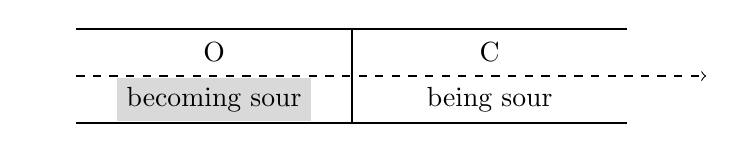
\begin{tikzpicture}[yscale=.2, xscale=.5]
    \node[fill=gray!30] at (5.5, 1.5) {becoming sour};
    \node at (12.5, 1.5) {being sour};
    \node at (1,3) {};
    \draw [thick] (2,0) -- (16,0);
    \draw [->, dashed] (2, 3) -- (18,3);
    \draw [thick] (2,6) -- (16,6);
    \draw [thick] (9, 0) -- (9, 6);
    \node at (5.5, 4.5) {O};
    \node at (12.5, 4.5) {C};
\end{tikzpicture}}
\ex\attop{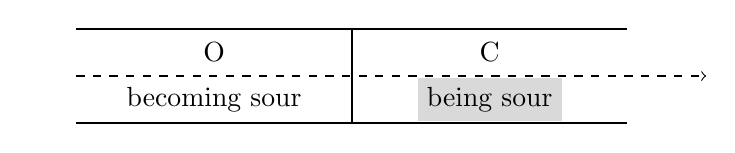
\begin{tikzpicture}[yscale=.2, xscale=.5]
    \node at (5.5, 1.5) {becoming sour};
    \node[fill=gray!30] at (12.5, 1.5) {being sour};
    \node at (1,3) {};
    \draw [thick] (2,0) -- (16,0);
    \draw [->, dashed] (2, 3) -- (18,3);
    \draw [thick] (2,6) -- (16,6);
    \draw [thick] (9, 0) -- (9, 6);
    \node at (5.5, 4.5) {O};
    \node at (12.5, 4.5) {C};
\end{tikzpicture}}
\end{xlist}
\end{exe}

                
All examples given in this section express a resultative reading, a reading which focuses on the present/ongoing state resulting from an event. This reading should not be confused with the perfect (of result) reading, a reading which focuses on the past event which resulted in a state of affairs, which in English can be exemplified by \textit{I} \textit{have} \textit{built} \textit{a} \textit{house} \textit{next} \textit{to} \textit{the} \textit{river}. Evidence that \textit{-ø-…-íle} in Nyamwezi denotes a resultative reading (in achievements), and \textit{not} a perfect of result, is its compatibility with -\textit{táá}- ‘still (being)’, which indicates that the result state of the situation still holds (is extended) \REF{ex:kanijo:17}. 

\ea \label{ex:kanijo:17}
\ea
    \glll a\textbf{taá}lɪ     agɪn\textbf{ílé}\\ 
    a-\textbf{táá}-lɪ   a-ø-gɪn-\textbf{íle}\\
    3\textsc{sg}-\textbf{still}-\textsc{aux} 3\textsc{sg}-become\_fat\textbf{-íle}\\
    \glt ‘s/he is still fat’

\ex  
    \glll a\textbf{taá}lɪ    amán\textbf{ílé}    kweendéésha βasikélí\\
    a-\textbf{táá}-lɪ       a-ø-man-\textbf{íle}    kʊ-endéésh-a βasikélí\\
    3\textsc{sg}-\textbf{still}-\textsc{aux} 3\textsc{sg}-get\_to\_know-\textbf{íle} \textsc{inf}-cycle-\textsc{fv}   bicycle \\
    \glt ‘S/he still knows how to ride a bicycle’
\z
\z

Co-occurrence of -\textit{táá}- ‘still (being)’ plus \textit{-ø-\ldots-íle} in Nyamwezi is a good piece of evidence for the resultative reading because resultatives, unlike perfects, in principle, are incompatible with ‘still’ (cf. \citealt{Dahl1985}:134). For example, in English *\textit{I} \textit{have} \textit{still} \textit{built} \textit{a} \textit{house} \textit{next} \textit{to} \textit{the} \textit{river} is not acceptable.  

 \subsection{\textit{-ø-…-íle} with statives}
 

In \figref{fig:kanijo:3}, it is stated that statives denote an indefinite state. These aspectual classes have no internal change; thus I argued that they lack a phasic structure. There are very few statives in Bantu languages in general, and in Nyamwezi in particular. Non-tense-marked statives in Nyamwezi denote a general present time reading; a reading in which the state of the situation having occurred is equivalent to the prior situation. For instance, all phases of the event \textit{asaatilé} ‘S/he is suffering’ in \REF{ex:kanijo:18} are identical. Whichever point of time we choose to cut in on this event, we shall find exactly the same situation. 

\ea \label{ex:kanijo:18}
\ea 
    \glll asaat\textbf{ilé}  kwɪɪngɪla  kʊβyaálwa  kwaákwé\\
    a-ø-saat-\textbf{íle}       kwɪɪngɪla kʊ-βyaál-w-a       kwaákwé\\
    3\textsc{sg}-be\_sick-\textbf{íle} since \textsc{inf}-bear-\textsc{pass}-\textsc{fv} \textsc{poss}\\
    \glt ‘S/he has been suffering since her birth.’

\ex 
    \glll   βatog\textbf{ilwé}          kʊ́βawɪ́ɪ́laa βiíchaaβó    βátʊmame\\       
            βa-ø-tog-\textbf{ílwe}    kʊ-βa-wɪɪl-a    a-βiíchaaβó     βá-tʊmám-eé\\          
    3\textsc{pl}-love-\textbf{íle}       \textsc{inf}-\textsc{oc}-tell-\textsc{fv} cl.1-companions\_their    cl.2-work-\textsc{opt}\\
  \glt ‘They like to tell their mates that they should work (hard).’
\z
\z

Statives in this language do not neatly indicate a cause-result relationship between the prior eventuality and the current state, thus both the progressive form -\textit{lɪɪ}- and the construction \textit{-ø-…-íle} give more or less the same interpretation, as shown in \REF{ex:kanijo:19}. 

\ea \label{ex:kanijo:19}
\ea 
    \glll ka\textbf{l}\textbf{ɪɪ}saata\\   
    ka-\textbf{lɪɪ}-saat-a\\                              
     cl.12-\textbf{\glossify{PROG}}-be\_sick-\textsc{fv}\\            
    \glt `S/he (small child) is sick.’         
\ex 
\glll kasaat\textbf{ilé}\\
ka-ø-saat-\textbf{íle}\\
cl.12-be\_sick-\textbf{íle}\\
\glt `S/he (small child) is sick.’ 
\z
\z

Although both \textit{-lɪɪ-} and \textit{-ø-\ldots-íle} receive the same translation in English, there is a difference having to do with whether an event is bounded or unbounded. The progressive form \textit{-lɪɪ-} suggests that the event holds at the moment of speaking but it will come to an end sometime in the future, whereas the construction \textit{-ø-\ldots-íle} does not give this implication. It just describes a (permanent) state. This distinction can be equated with \citegen{Kratzer1995} distinction between stage-level statives which refer to temporary states and individual-level statives which refer to permanent states. Schematically, the difference between \textit{-lɪɪ-} and \textit{-ø-\ldots-íle} is shown in Figures~\ref{fig:kanijo:7} and \ref{fig:kanijo:8}, where a bold vertical line indicates boundedness of an event in \figref{fig:kanijo:7} (stage level). The lack of this line in \textup{\figref{fig:kanijo:8}} implies the event is unbounded (individual-level). 


\begin{figure}
\begin{tikzpicture}[xscale=.5, yscale=.2]
    \node[fill=gray!50] at (4,0) {ka-lɪɪ-saat-a};
 \draw[ultra thick] (9, 0) -- (9, 6);
 \draw[dashed] (0, 3) -- (8, 3);
\end{tikzpicture}
\caption{\textit{‑lɪɪ-} event structure\label{fig:kanijo:7}}
\end{figure}

\begin{figure}
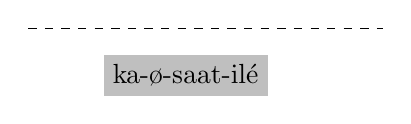
\begin{tikzpicture}[xscale=.5, yscale=.2]
    \node[fill=gray!50] at (4,0) {ka-ø-saat-ilé};
 \draw[dashed] (0, 3) -- (9, 3);
\end{tikzpicture}
\caption{\textit{-ø-…-íle} event structure\label{fig:kanijo:8}}
\end{figure}

It is hard to find a context where the difference between -\textit{lɪɪ-} and \textit{-ø-…-íle} occurs. One of the language consultants for this study mentioned that in many contexts he can use both ways to express the same meaning. The difficulty in finding a context where one can appreciate the difference between the two formatives lies in the fact that the situation of getting sick for instance, which for the case of achievements can be selected by the progressive, is equal to the current state (which in achievements is picked out by the \textit{-ø-…-íle}). Statives do not show this type of relationship.

In order to find the difference, consultants were asked to tell which of the two forms they can use when talking about chronic diseases. They all agreed that the construction \textit{-ø-…-íle} is appropriate when talking about chronic diseases (hence unacceptable in 20b), while the form -\textit{lɪɪ-} is only used to talk about curable diseases like malaria (hence acceptable in 20a). The use of \textit{-ø-…-íle} when referring to chronic diseases gives some evidence that this construction really describes a state, while -\textit{lɪɪ-} denotes an event which is true for the time being, but probably it will not persist in the coming days. 

\ea{}\label{ex:kanijo:20}
[Context: Someone has arrived and is looking at the children who are playing at the house compound. As she was expecting to see J, but J is not there, she then asks “where is J today?”] 

\ea[*]{ \glll waaláálaga    \`{m}kaaya,              asaat\textbf{ilé}           málelíyá\\
       ʊ-á-laál-ag-a                \`{m}-kaaya,            a-ø-saat-\textbf{íle}      malelíyá\\
       3\textsc{sg}-\textsc{cpl}-sleep-\textsc{rec}-\textsc{fv} \textsc{loc}-homestead 3\textsc{sg}-be\_sick-\textbf{íle} malaria\\
       \glt ‘She is sleeping inside the house, suffering from malaria.’}


 \ex[]{\glll waaláálaga \`{m}kaaya, a\textbf{l}\textbf{ɪɪ}saata  malelíyá\\
      ʊ-á-laál-ag-a             mu-kaaya,      a-\textbf{lɪɪ}-saat-a                malelíyá\\
       3\textsc{sg}-\textsc{cpl}-sleep-\textsc{rec}-\textsc{fv} \textsc{loc}-homestead 3\textsc{sg}-\textbf{\textsc{prog}}-be\_sick-\textsc{fv} malaria\\
      \glt ‘She is sleeping inside the house, suffering from malaria.’}
\z
\z

\subsection{\textit{-ø-…-íle} with activities, classified as ``directed motion verbs''}\label{sec:kanijo:4.3}

As described in the previous section, duratives, in general, have an extended nuclear phase (as shown in \figref{fig:kanijo:9}). Duratives are classified into two subclasses: activities (those in which the nuclear phase indicates internal change of an event from moment to moment, e.g. -\textit{lyaá} ‘eat’ and \textit{-peela} ‘run’) and serial semelfactives (those in which the nuclear phase constitutes multiple occurrences of a situation when perceived as series, e.g. -\textit{kolola} ‘laugh’). 

\begin{figure}
\caption{Durative event\label{fig:kanijo:9}}
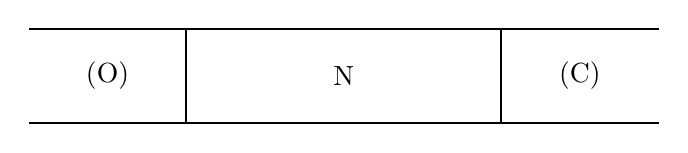
\begin{tikzpicture}[yscale=.2, xscale=.5]
{
\draw [thick] (0,0) -- (16, 0);
\draw [thick] (0, 6) -- (16, 6);
\draw [thick] (4, 0) -- (4, 6);
\draw [thick] (12, 0) -- (12, 6);
\node at (2, 3) {(O)};
\node at (14, 3) {(C)};
\node at (8, 3) {N};
};
\end{tikzpicture}
\end{figure} 

In the discussion of activity verbs in \sectref{sec:kanijo:3.2}, I stated that motion verbs with directional interpretation and a goal (called directed motion verbs), e.g. \textit{-peela} ‘run (to the store)’, behave somewhat differently from other duratives. These verbs in \citeauthor{Botne2000}'s model do not specify the coda phase, a phase at which a result state comes about. So, they are schematically represented in \figref{fig:kanijo:10} where the last phase is nuclear phase. 


\begin{figure}
\caption{Event structure for directed motion verbs\label{fig:kanijo:10}}

\begin{tikzpicture}[yscale=.2, xscale=.5]
{
\draw [thick] (0,0) -- (16, 0);
\draw [thick] (0, 6) -- (16, 6);
\draw [thick] (8, 0) -- (8, 6);
\node at (4, 3) {(O)};
\node at (12, 3) {N};
};
\end{tikzpicture}
\end{figure}

We saw in example \REF{ex:kanijo:16} that in aspectual classes which encode a resultant/coda phase, \textit{-ø-…-íle} picks out this phase and gives a resultative reading. Since in directed motion verbs the coda phase is not part of the situation’s event (see \figref{fig:kanijo:10}), \textit{-ø-…-íle} picks out the nuclear phase and gives a reading which can be translated with progressive form in English (progressive-like reading) \REF{ex:kanijo:21}. \citet[194]{Ebert1995} notes a similar phenomenon in Arabic where what is called the ``Active Particle'' form, which usually indicates perfect/resultative meaning in other verbs, in verbs of posture, of motion and of sensory perception expresses a progressive-like reading.

It is important to state that \textit{-ø-…-íle} in both achievements and directed motion verbs is attuned to the initial (left) edge of the nuclear phase. This means that in achievements the perspective is in the stative coda phase, but in directed motion verbs it is in the nuclear phase.

\ea \label{ex:kanijo:21}
\ea
\glll apeel\textbf{ilé}  kʊjaa kʊmadʊʊka\\
 a-ø-peel-\textbf{íle} kʊ-j-a kʊ-madʊʊka\\
   3\textsc{sg}-run-\textbf{íle} \textsc{inf}-go-\textsc{fv} \textsc{loc}-shops\\
 \glt ‘S/he is/has run off to the shops.’

\ex 
\glll  gaángɪ     gííz\textbf{ilé}  nágaángɪ  gáshook\textbf{ílé}\\
 ga-ángɪ     ga-ø-iz-\textbf{íle}      na-gaángɪ  ga-shook-\textbf{íle}\\
 cl.6-other  cl.6-come-\textbf{íle} and-other   cl.6-return-\textbf{íle}\\
\glt ‘Some (e.g. lions in a narration) are coming and some are going back.’
\z
\z

The progressive-like reading in directed motion verbs, as exemplified above, is also a resultative in its function, just like that of achievements. The progressive reading in these verbs is a matter of the English translation (cf. \citealt{Ebert1995}:189). The difference between a resultative reading of achievements and that of directed motion verbs is that, in achievements the result state is triggered by a nuclear phase which denotes the change-of-state, whereas in directed motion verbs the initial point (onset phase) is regarded as a point of change (cf. \citealt{Smith1991}:70). Since the phase following this point of transition in directed motion verbs is a nuclear phase, \textit{-ø-…-íle} selects this ongoing/dynamic non-stative phase to encode a stative(-like) meaning along the lines of ‘be directed towards a certain goal’. 

One piece of evidence is present to justify the claim that directed motion verbs encode a kind of change-of-state which is similar to that of achievements. Both directed motion verbs, as shown in \REF{ex:kanijo:22}, and achievements (see e.g. \ref{ex:kanijo:17} repeated in \REF{ex:kanijo:23}) occur with the persistive form -\textit{táá}- ‘still (being)’ plus \textit{-ø-…-íle}. Co-occurrence of this construction with directed motion verbs indicates that a state that results from an ongoing situation still holds.

\ea \label{ex:kanijo:22}
\glll a\textbf{taá}lɪ  alɪ  \`{m}nzɪla  az\textbf{ííl}é kaayá\\
  a-\textbf{táá}-lɪ           a-lɪ           mu-nzɪla  a-j-\textbf{íle}        kaayá\\
  3\textsc{sg}-\textbf{still}-\textsc{aux} 3\textsc{sg}-COP \textsc{loc}-path 3\textsc{sg}-go-\textbf{íle} home\\
\glt   ‘S/he is on the way (going) home’
\z

\ea \label{ex:kanijo:23}
\glll a\textbf{taá}lɪ              agɪn\textbf{ílé} \\
  a-\textbf{táá}-lɪ            a-ø-gɪn-\textbf{íle}\\
  3\textsc{sg}-\textbf{still}-\textsc{aux} 3\textsc{sg}-become\_fat-\textbf{íle}\\
\glt   ‘S/he is still fat’
\z


In directed motion verbs, English makes no distinction between the progressive form \textit{-lɪɪ-} and \textit{-ø-…-íle}. So, both \textit{a-lɪɪ-peel-a} and \textit{a-peel-ilé} are translated in English as ‘s/he is running’. The difference between \textit{-lɪɪ-} and \textit{-ø-…-íle}, however, can be settled by context. For instance, in \REF{ex:kanijo:24}, the context is such that the speaker is watching a movie but he missed a part in the movie where the actress (Kajala) saw a lion and started to run away. He then asks another person who started to watch the movie before he came “Why is Kajala running away?” (\textit{kʊʊngʊno-kɪ} \textit{ʊ-kajala a-lɪɪ-peel-a?}). A response to this question with the progressive form \textit{-lɪɪ-} sounds fine (\ref{ex:kanijo:24}a), but one with \textit{-ø-…-íle} sounds odd (\ref{ex:kanijo:24}b). 

\ea \label{ex:kanijo:24}
\ea[]{ 
\glll a\textbf{l}\textbf{ɪɪ}peel’ iishiímbá\\
  a-\textbf{lɪɪ}-peel-a              i-shiímbá\\
 3\textsc{sg}-\textbf{\textsc{prog}}-run-\textsc{fv} cl.5-lion\\
\glt  ‘She is fleeing from a lion’ (Lit: ‘She is running away from the lion’)}

\ex[*]{\glll apeel\textbf{il}’       ííshiímbá\\
   a-ø-peel-\textbf{íle} i-shiímbá\\
   3\textsc{sg}-run-\textbf{íle}   cl.5-lion\\
  \glt ‘She fled from a lion’ (Lit: ‘She is running away from the lion’)}
\z
\z

Likewise, the progressive form \textit{-lɪɪ-} cannot be used to refer to the continuing state of the subject, which is encoded by \textit{-ø-…-íle}. For instance, \REF{ex:kanijo:25} is in a context where the teacher is looking for a missing student (Anna). He then asks other students who were outside the class playing, “Have you seen Anna today?” (\textit{w-aa-mú-βon-ág-a} \textit{ʊ-ana} \textit{leeloó?}). A response to this question with the progressive form \textit{-lɪɪ-} sounds odd (\ref{ex:kanijo:25}b), but one with \textit{-ø-…-íle} sounds fine (\ref{ex:kanijo:25}a).

\ea \label{ex:kanijo:25}
\ea[]{ \glll waaβɪtaga                   apeel\textbf{ilé}\\
\textbf{    }ʊ-á-βɪt-ag-á                 a-ø-peel-\textbf{íle}\\
 3\textsc{sg}-\textsc{cpl}-pass-\textsc{rec}-\textsc{fv} 3\textsc{sg}-\textsc{prog}-run-\textbf{íle}\\
\glt  ‘She passed (here) running.’}

\ex[*]{\glll waaβɪtaga                   a\textbf{l}\textbf{ɪɪ}peela\\
   ʊ-á-βɪt-ag-á                a-\textbf{lɪɪ}-peel-a\\
   3\textsc{sg}-\textsc{cpl}-pass-\textsc{rec}-\textsc{fv} 3\textsc{sg}-\textbf{\textsc{prog}}-run-\textsc{fv} \\
\glt    She passed (here) running’}
\z
\z

The co-occurrence of the \textit{-lɪɪ-} and \textit{-ø-…-íle} in the same construction provides further evidence that the two forms do not perform the same function. One (\textit{-ø-…-íle}) indicates a state and the other (\textit{-lɪɪ-}) indicates the action in progress. This distinction is illustrated in \REF{ex:kanijo:26} where the point of speech is now, the point of reference is in the past, established by -\textit{βɪtá} ‘pass’, continued by \textit{-peela} ‘run’ and directed towards a location by -\textit{ja} ‘go’. The continuation of the event of running can be construed as a dynamic state (\ref{ex:kanijo:26}a) or a process (\ref{ex:kanijo:26}b). Similarly, \textit{-ja} ‘go’ which indicates the direction of the event can be construed as a process (\ref{ex:kanijo:26}a) or a dynamic state (\ref{ex:kanijo:26}b). This relationship is further expressed by literal translations. 

\ea \label{ex:kanijo:26}
\ea
\glll waaβɪtaga apeel\textbf{ilé}, a\textbf{l}\textbf{ɪɪ}ja kaaya \\
    ʊ-á-βɪt-ag-á                a-ø-peel-\textbf{íle}, a-\textbf{l}ɪɪ-j-a                 kaaya \\
    3\textsc{sg}-\textsc{cpl}-pass-\textsc{rec}-\textsc{fv} 3\textsc{sg}-run-\textbf{íle}  3\textsc{sg}-\textbf{\textsc{prog}}-go-\textsc{fv} homestead \\
\glt    Lit. ‘She passed (here), she was running going home’ \\
   ‘She passed (here), having run, going home.’
\ex
\glll waaβɪtaga a\textbf{l}\textbf{ɪɪ}peela, az\textbf{íílé}         kaáya\\
    ʊ-á-βɪt-ag-á                 a-\textbf{l}ɪɪ-peel-a            a-z-\textbf{íle}       kaaya\\
    3\textsc{sg}-\textsc{cpl}-pass-\textsc{rec}-\textsc{fv} 3\textsc{sg}-\textbf{\textsc{prog}}-run-\textsc{fv} 3\textsc{sg}-go-\textbf{íle} homestead\\
    \glt Lit. ‘She passed (here) running, s/he was going home’\\
    ‘She passed (here) running, gone off home.’
\z
\z

Another piece of evidence is that neither the progressive form \textit{-lɪɪ-}, as in (\ref{ex:kanijo:27}a), nor the construction \textit{-ø-…-íle}, as in (\ref{ex:kanijo:27}b), can be used with both -\textit{peela} ‘run’ and -\textit{ja} ‘go’, as each form performs a different function in Nyamwezi. 

\ea \label{ex:kanijo:27}
\ea[*]{
\glll waaβɪtaga a\textbf{l}\textbf{ɪɪ}peela,  a\textbf{l}\textbf{ɪɪ}ja kaaya\\
      ʊ-á-βɪt-ag-á                 a-\textbf{lɪɪ}-peel-a             a-\textbf{lɪɪ}-j-a kaaya\\
      3\textsc{sg}-\textsc{cpl}-pass-\textsc{rec}-\textsc{fv} 3\textsc{sg}-\textbf{\textsc{prog}}-run-\textsc{fv} 3\textsc{sg}-\textbf{\textsc{prog}}-go-\textsc{fv}  homestead\\
      \glt    Lit. ‘She passed (here) she was running, s/he was going home’\\
   ‘She passed here, she was running towards home’}
\ex[*]{\glll waaβɪtaga apeel\textbf{ilé}       az\textbf{íílé}        kaáya\\
    ʊ-á-βɪt-ag-á                a-ø-peel-\textbf{íle} a-z-\textbf{íle}       kaaya\\
    3\textsc{sg}-\textsc{cpl}-pass-\textsc{rec}-\textsc{fv} 3\textsc{sg}-run-\textbf{íle} 3\textsc{sg}-go-\textbf{íle} homestead \\
\glt  Lit. ‘She passed (here) running, going home’\\
    ‘She passed here, she was running towards home.’}
\z
\z

\subsection{\textit{-ø-…-íle} with other activities and semelfactives} \label{sec:kanijo:4.4}

In the previous section, I argued that directed motion verbs in Nyamwezi behave somewhat differently from other activity verbs and (serial) semelfactives. Directed motion verbs, as we have seen, do not lexically encode the (resultant state) coda phase, they only encode an optional onset phase and a nuclear phase. In directed motion verbs, \textit{-ø-…-íle} selects the nuclear phase and gives a progressive-like reading.

Another category of activity verb includes verbs such as -\textit{sha} ‘grind (e.g. corn)’, \textit{-dɪtɪla} ‘pour (e.g. water) into (a receptacle)’, -\textit{pʊʊla} ‘pound (e.g. corn)’, -\textit{zeenga} ‘build (e.g. a house)’ -\textit{lɪma} ‘cultivate (e.g. a farm)’ and -\textit{chiβá} ‘block hole/way, plug’, which, compared to directed motion verbs, lexically indicates a durative nucleus and an entailed resultant/coda state (cf. \citegen{Persohn2017b} processes with a resultant state). In many of these verbs in Bantu languages, -\textit{íle} tends to pick out a resultant/coda state phase to give a perfect of result reading (see e.g. Luwanga and Lusaamia in \citet{Botne2010}) or resultative reading (see e.g. Totela in \citet{Crane2013}). The same is also observed in Nyamwezi, verbs such as -\textit{sha} ‘grind’ and \textit{-dɪtɪla} ‘pour into’, as exemplified in (\ref{ex:kanijo:28}a) and (\ref{ex:kanijo:28}b), respectively, occur with \textit{-ø-…-íle} to encode a patientive resultative reading. In this reading, the verb’s subject, which has the semantic role of the patient (patientive subject), undergoes a change-of-state. Note that some verbs in this category permit the causative alternation in which the patientive resultative reading is triggered by both \textit{-ø-…-íle} and the passive form -\textit{w}- (\ref{ex:kanijo:28}c), though some take the passive form but do not allow causative alternation (\ref{ex:kanijo:28}d--e)\footnote{For comparison, an example below indicates a sentence with agent-verb-patient S-V-O structure in Nyamwezi.       
\begin{exe}
\ex \glll ʊkúlwá alɪɪshaa ŋhalaanga\\
ʊ-kúlwá  a-lɪɪ-sh-a         ŋhalaanga\\
A-kulwa 3\textsc{sg}-\textsc{PROG}-grind-\textsc{\textsc{fv}} peanuts\\
\glt `Kulwa grinds (is grinding) peanuts'\\
\end{exe}}. For the purpose of this study, I will not go into detail to discuss the question why some verbs in this category permit causative alternation while others do not. Further studies are required on the lexical semantics of these verbs. 

\ea \label{ex:kanijo:28}
\ea
\glll  *ash\textbf{iílé}        vs.   zish\textbf{iílé}\\
\textbf{ }a-ø-sh-\textbf{íle}   {}    zi-ø-sh-\textbf{íle}\\
 3\textsc{sg}-grind-\textbf{íle}  {}      cl.10-grind-\textbf{íle}\\
 \glt ‘S/he has ground (the peanuts)’  {}  ‘They (peanuts) are ground.’
\ex \glll *adɪtɪl\textbf{ílé}      vs.  yɪdɪtɪl\textbf{ílé}\\
a-ø-dɪtɪl-\textbf{íle}   {}   yɪ-ø-dɪtɪl-\textbf{íle}\\
3\textsc{sg}-pour\_into-\textbf{íle}  {}  cl.9-pour into-\textbf{íle}\\
\glt ‘S/he has poured (water) into a vessel.’ {} ‘It (a vessel) has been poured into’.

\ex \glll achiβ\textbf{ílé}      vs.  yɪchiβ\textbf{íl}w\textbf{é} (*yɪchiβ\textbf{ílé})\\
    a-ø-chiβ-\textbf{íle}   {}   yɪ-ø-chiβ-\textbf{íl}-\textbf{w}-\textbf{e}\\
    3\textsc{sg}-block-\textbf{íle}  {}   cl.9-block-\textbf{\textsc{pass}-íle}\\
    \glt ‘S/he has closed (a way)’ {} ‘It (the way) is closed’

\ex \glll *apʊʊl\textbf{ílé}      vs.  gapʊʊl\textbf{íl}w\textbf{é} (*gapʊʊl\textbf{ílé})\\
    a-ø-pʊʊl-\textbf{íle}   {}   ga-ø-pʊʊl-\textbf{íl-w-e}\\
    3\textsc{sg}-pound-\textbf{íle}  {}    cl.6-pound-\textbf{\textsc{pass}-íle}\\
\glt     ‘S/he has pounded (the corn)’ {} ‘It (corn) is pounded’

\ex \glll *alɪm\textbf{ilé}      vs.  lɪlɪm\textbf{ilwé}\\
a-ø-lɪm-\textbf{íle}    {}    lɪ-ø-lɪm-\textbf{íl-w-e}\\
3\textsc{sg}-cultivate-\textbf{íle}  {}    3\textsc{sg}-cultivate-\textbf{\textsc{pass}}-\textbf{íle}\\
\glt ‘She has cultivated (a farm.)’ {} ‘It (a farm) is cultivated’
\z
\z

Verbs shown above are subject to a second type of result state analysis which is similar to that of achievements. The resultant state in these verbs involves a “durative transition” from one state to another, whereas in achievements the change is thought of as occurring instantaneously (cf. \citealt{Pustejovsky1991}).

So far, we have discussed two categories of activity verbs, i.e. those which do not lexically encode a resultant/coda phase (directed motion verbs), and those activity verbs which typically entail a resultant/coda state and suggest a change-of-state of the verb’s patientive subject. Another category of verbs includes verbs such as -\textit{lila} ‘cry’ and -\textit{seka} ‘laugh’, which resemble directed motion verbs in encoding an optional onset phase and a nuclear phase without a resultant/coda phase. \textit{-ø-…-íle} in general does not occur with these verbs without additional context. The context where the interaction of \textit{-ø-…-íle} with verbs such as -\textit{seka} ‘laugh’ is accepted is when the speaker needs to show her/his ability towards what has been conceived impossible by other people. For example, in \REF{ex:kanijo:29}, the speaker may use \textit{-ø-…-íle} to mean that s/he has the ability to make the person referred to laugh (something which no one else did). 

\ea \label{ex:kanijo:29}
\ea
\glll ʊkʊwaaneé    asek\textbf{ílé}\\
  ʊ-kʊ-waaneé a-ø-sek-\textbf{íle}\\
   A-\textsc{loc}-\textsc{poss}  3\textsc{sg}-laugh-\textbf{íle}\\
  \glt ‘To me, s/he must laugh (just wait and see)’
\z
\z

In \REF{ex:kanijo:28}, we saw that -\textit{sha} ‘grind’, \textit{-dɪtɪla} ‘pour into’, and -\textit{pʊʊla} ‘pound’ do not naturally occur with \textit{-ø-…-íle} if the verb’s subject has the semantic role of agent (agentive subject). However, the speaker can use \textit{-ø-…-íle} if s/he wants to express a contradiction and/or emphasis in the similar way as verbs without an entailed resultant/coda phase. This is contextualized in \REF{ex:kanijo:30} using the verb -\textit{lɪma} ‘cultivate’.\pagebreak

\ea \label{ex:kanijo:30}
[Context: It is a rainy season, Benny is uncertain whether his brother Frank has cultivated. While talking with his neighbors, he says “I wonder whether Frank has cultivated this season or whether he even has a farm” If one of the neighbors is sure that Frank has cultivated s/he can respond using \textit{-ø-…-íle}.]

\glll alɪm\textbf{ilé}\\
a-ø-lɪm-\textbf{íle}\\
3\textsc{sg}-cultivate-\textbf{íle}\\
\glt ‘He has cultivated (and I saw his farm.)’
\z

In all verbs where \textit{-ø-…-íle} is not acceptable without context, I argue that \textit{-ø-…-íle} is coerced to occur with these verbs in order to express a contrast\slash contradiction and/or emphasis. \citet{Collins1962}, as cited in \citet[70]{Crane2012}, reports a similar phenomenon in Tonga, where -\textit{ide} (another variant of -\textit{ile}) is used to express contradiction \REF{ex:kanijo:31}. See also \citet{Woidich1975}, as cited in \citet[194]{Ebert1995}, for a marker of resultative expressing emphasis. 

\ea \label{ex:kanijo:31}  (\citealt{Collins1962}, as cited in \citealt{Crane2012}:70)\\
micelo ili bolede (-\textit{bola} ‘become rotten’)
\glt   ‘the fruits are rotten, or the fruits are \textit{not} perfectly sound’ 
\z

According to \citet{Collins1962}, the sentence in \REF{ex:kanijo:31} would be used in argument or to express disappointment or surprise. 

The use of \textit{-ø-…-íle} in Nyamwezi to express contradiction\slash emphasis is different from that of a stativizer which gives readings such as resultative/stative and progressive-like. Contradiction and/or emphasis can be regarded as a second main function of -\textit{ø-…-íle} which is enforced by context. 

Let’s now turn to the discussion of the interaction of semelfactives with -\textit{ø}-…-\textit{íle}. In all contexts attested during elicitation sessions, -\textit{ø}-…-\textit{íle} was not accepted with serial semelfactives. Since (serial) semelfactives resemble activities in encoding an extended nuclear phase, one of the ways to test co-occurrence of -\textit{ø}-…-\textit{íle} with semelfactives was to see if the interaction would lead to the progressive-like reading. To try this, the consultants were asked to say whether they would use \textit{a-ø-kolol-ílé} (from \textit{-kolola} ‘cough’) to mean that someone is coughing. The example meant to check if the sentence may get an iterative interpretation (several instances of an event within a measurable duration) \REF{ex:kanijo:32a} or denote periodic events \REF{ex:kanijo:32b}. Both interpretations were rejected. 

\ea \label{ex:kanijo:32}
\ea[*]{  \glll a\textbf{taá}lɪ\'{}       akolol\textbf{ílé} \label{ex:kanijo:32a}\\
      a-\textbf{táá-}lɪ            a-ø-kolol-\textbf{íle}\\
      3\textsc{sg}-\textbf{still}-\textsc{aux} 3\textsc{sg}-cough-\textbf{íle}\\
      \glt ‘S/he is still coughing (continuously)}

\ex[*]{  \glll akolol\textbf{ílé}         kʊfúma mázʊʊlí \label{ex:kanijo:32b}\\
      a-ø-kolol-\textbf{íle}    kʊfuma mazʊʊlí\\
      3\textsc{sg}-cough-\textbf{íle} since     {day before yesterday}\\
\glt ‘S/he has been coughing since the day before yesterday’}
\z
\z


  Semelfactives cannot occur with -\textit{ø}-…-\textit{íle}, even though they encode a kind of extended nuclear phase which can be picked out by this construction. One of the reasons for the co-occurrence restriction is that for a verb which does not naturally occur with -\textit{ø}-…-\textit{íle} it needs a context where this formative can be coerced to occur with that verb. Coercion of -\textit{ø}-…-\textit{íle} normally suggests a contradiction/emphasis. For this reason, it is very awkward for a speaker to use -\textit{ø}-…-\textit{íle} with semelfactives to imply that s/he has the ability to enforce the occurrence of, let us say, ‘cough’ which is difficult to do to other people, in the same way it is possible with -\textit{seka} ‘laugh’ in \REF{ex:kanijo:29}. So, the co-occurrence restriction is due to the inability of the speaker to enforce events denoted by semelfactives. Otherwise, if the speaker believes that s/he has the ability to enforce a semelfactive event (as in a non-literal context), then s/he may use -\textit{ø}-…-\textit{íle}. 


To conclude this section, \textit{-ø-…-íle}, in general, does not commonly occur with activity verbs. The co-occurrence is subject to two conditions (i) the verb denotes a result state that leads to the change-of-state/condition of the verb’s patientive subject, and (ii) the verb is used in a special pragmatic condition where \textit{-ø-…-íle} is coerced to express contradiction and/or emphasis.

\section{Conclusion}\label{sec:kanijo:5}\largerpage[-2]

To summarize, the paper has generally shown that the analysis of aspectual classes is crucial in understanding the functions of \textit{-ø-…-íle} in Nyamwezi. A resultative reading occurs with achievements, a general present time reading occurs with statives, and a progressive-like reading occurs with a handful of activity verbs called directed motion verbs. It was also shown that there are some activity verbs, apart from directed motion verbs, which occur quite naturally with \textit{-ø-…-íle}. These verbs share some commonalities with achievements, as they both lead to the change-of-state of the verb’s patientive subject. More importantly, it was noted that, activity verbs which lack an entailed resultant/coda phase, in special pragmatic contexts, can be coerced to occur with \textit{-ø-…-íle} to express contrast/contradiction and/or emphasis. It was also argued that although coercion seems to be an option in contexts where \textit{-ø-…-íle} is not allowed with some verbs, this is not the case with semelfactives. Coercion of \textit{-ø-…-íle} with semelfactive verbs in general is not allowed due to the inability of the speaker to enforce events denoted by semelfactives. 

In short, \textit{-ø-…-íle} in Nyamwezi has two main functions: (i) statitivizer, which leads to three readings -- resultative, general present time and progressive-like -- and (ii) contradiction/emphasis. These results suggest that in other Bantu languages a more detailed analysis of \textit{-íle} can yield valuable results, which may previously have gone unnoticed.  

%@incollection{Bar-el2015,
%	address = {Oxford},
%	author = {Bar-el, Leora},
%	booktitle = {Methodologies in Semantic Fieldwork (pp.},
%	editor = {M. Ryan Bochnak & Lisa Matthewson},
%	pages = {75–109},
%	publisher = {Oxford University Press},
%	title = {Documenting and Classifying Aspectual Classes Across Languages},
%	year = {2015}
%}


%Botne, Robert. (1983). On the notion “inchoative verb” in Kinyarwanda. Le Kinyarwanda, langue bantu du Rwanda - Études linguistiques, 149–180.

%@book{Botne2008a,
%	address = {Philadelphia},
%	author = {Botne, Robert.},
%	publisher = {American Philosophical Society},
%	title = {A grammatical sketch of Chindali (Malawian variety)},
%	year = {2008}
%}


%Botne, Robert. (2010). Perfectives, perfect and pasts, oh my!: On the semantics of -ILE in Bantu. Africana Linguistica(16), 31–63.

%@article{Botne2000,
%	author = {Botne, Robert,  and  Kershner, Tiffany L},
%	journal = {Afrika und Übersee},
%	pages = {161–180},
%	title = {Time, tense and the perfect in {Zulu}},
%	volume = {83},
%	year = {2000}
%}


%Brisard, Frank, & Meeuwis, Michael. (2009). Present and perfect in Bantu: The case of Lingála. Journal of African Languages and Linguistics(30), 21–43.

%@book{Bybee1994,
%	address = {Chicago},
%	author = {Bybee, Joan, Perkins, Revere,  and  Pagliuca, William},
%	publisher = {The University of Chicago Press},
%	title = {The evolution of grammar: {{T}}ense, aspect and modality in the languages of the world},
%	year = {1994}
%}


%@book{Comrie1976,
%	address = {Cambridge},
%	author = {Comrie, Bernard.},
%	publisher = {Cambridge University Press},
%	title = {Aspect: {{A}}n introduction to the study of verbal aspect and related problems},
%	year = {1976}
%}


%@article{Crane2012,
%	author = {Crane, Thera Marie},
%	journal = {Africana Linguistica},
%	pages = {41--96},
%	title = {-ile and the pragmatic pathways of the resultative in {Bantu} Botatwe},
%	volume = {18},
%	year = {2012}
%}


%@article{Crane2013,
%	author = {Crane, Thera Marie},
%	journal = {Lingua},
%	note = {doi:http://dx.doi.org/10.1016/j.lingua.2013.04.006},
%	pages = {164--188},
%	title = {Resultatives, progressives, statives, and relevance: {{T}}he temporal pragmatics of the -ite suffix in {Totela}},
%	volume = {133},
%	year = {2013}
%}


%Crane, Thera Marie, & Fleisch, Axel. (2016). Event type lexicalization across language boundaries. Verbs in South African Ndebele varieties. Paper presented at the Bantu 6, University of Helsinki, June 20–22 2016. http://blogs.helsinki.fi/bantu-6/files/2016/09/Bantu6-CraneFleisch-Event-Type-Lexicalization-Across-Language-Boundaries.pdf

%@book{Dahl1985,
%	address = {Oxford},
%	author = {Dahl, Östen.},
%	publisher = {Blackwell},
%	title = {Tense and aspect systems},
%	year = {1985}
%}


%Ebert, Karen. (1995). Ambiguous perfect-progressive forms across languages. In Pier-Marco Bertinetto, Valentina Bianchi, Osten Dahl, & Mario Squartini (Eds.), In: Temporal reference, aspect, and actionality (Vol. 2). Torino: Rosenberg & Sellier.

%@incollection{Filip2012,
%	address = {Oxford},
%	author = {Filip, Hana},
%	booktitle = {The {Oxford} handbook of tense and aspect (pp.},
%	editor = {Robert. I Binnick},
%	pages = {721--751},
%	publisher = {Oxford University Press},
%	title = {Lexical aspect},
%	year = {2012}
%}


%@book{Freed1979,
%	address = {Dordrecht},
%	author = {Freed, Alice.},
%	publisher = {D. Reidel Publishing Company},
%	title = {The semantics of {English} Aspectual complementation},
%	year = {1979}
%}


%Guthrie, Malcolm. (1967–1971). Comparative Bantu: An introduction to the comparative linguistics and prehistory of the Bantu languages (Vol. 1-4). London: Gregg International Publishers.

%@book{Kearns2000,
%	address = {New York},
%	author = {Kearns, Kate.},
%	publisher = {Palgrave Macmillan},
%	title = {Semantics},
%	year = {2000}
%}


%@book{Kershner2002,
%	address = {The verb in Chisukwa},
%	author = {Kershner, Tiffany Lynne.},
%	publisher = {Aspect, tense, and time. (Ph.D. thesis), Indiana University},
%	title = {\biberror{no title}},
%	year = {2002}
%}


%Kratzer, Angelika. (1995). Stage-Level and Individual-Level predicates. In Gregory N. Carlson & Francis Jeffry Pelletier (Eds.), The Generic Book (pp. 125 - 175). Chicago: Chicago University Press.

%@book{Lewis2013,
%	address = {Ethnologue},
%	author = {Leclerc, Jacques.},
%	note = {//www.ethnologue.com/language/nym},
%	publisher = {Languages of the World, SIL International.   Retrieved from https:},
%	title = {\biberror{no title}},
%	year = {2013}
%}


%@book{Maganga1992,
%	address = {Köln},
%	author = {Maganga, Clement,  and  Schadeberg, Thilo.},
%	publisher = {Rüdiger Köppe},
%	title = {Kinyamwezi: {{G}}rammar, texts, vocabulary},
%	year = {1992}
%}


%@misc{Masele2001,
%	author = {Masele, Balla F. Y.P},
%	title = {The linguistic history of Sisuumbwa, Kisukuma and Kinyamweezi in {Bantu} zone F. {{P}}hD dissertation. {{M}}emorial University of Newfoundland.},
%	year = {2001}
%}


%@book{Nurse2008,
%	address = {Oxford},
%	author = {Nurse, Derek.},
%	publisher = {OUP},
%	title = {Tense and aspect in {Bantu} languages},
%	year = {2008}
%}


%@book{Persohn2017,
%	address = {Aspectuality in Bantu},
%	author = {Persohn, Bastian.},
%	publisher = {On the limits of Vendler’s categories. Linguistic Discovery, 15. (accepted)},
%	title = {\biberror{no title}},
%	year = {2017a}
%}


%@book{Persohn2017,
%	address = {Berlin},
%	author = {Persohn, Bastian.},
%	publisher = {Language Science Press},
%	title = {The verb in {Nyakyusa}: {{A}} focus on tense, aspect and modality},
%	year = {2017b}
%}


%@article{Pustejovsky1991,
%	author = {Pustejovsky, James},
%	journal = {Cognition},
%	pages = {47–81},
%	title = {The syntax of event structure},
%	volume = {41},
%	year = {1991}
%}


%@book{Rothstein2004,
%	address = {Oxford},
%	author = {Rothstein, Susan.},
%	publisher = {Blackwell Publishing},
%	title = {Structuring events: {{A}} study in the semantics of lexical aspect},
%	year = {2004}
%}


%@article{Sasse2002,
%	author = {Sasse, Hans-Jürgen},
%	journal = {Recent activity in the theory of aspect: Accomplishments, achievements, or just non-progressive state? Linguistic Typology},
%	number = {6},
%	pages = {199–271},
%	title = {\biberror{no title}},
%	volume = {2},
%	year = {2002}
%}


%@book{Seidel2008,
%	address = {Cologne},
%	author = {Seidel, Frank.},
%	publisher = {Rüdiger-Köppe Verlag},
%	title = {A grammar of Yeyi: {{A}} {Bantu} language of Southern Africa},
%	year = {2008}
%}


%@book{Smith1991,
%	address = {Dordrecht},
%	author = {Smith, Carlota S.},
%	publisher = {Kluwer Academic Publishers},
%	title = {The Parameter of Aspect},
%	year = {1991}
%}


%@article{Vendler1957,
%	author = {Vendler, Zeno},
%	journal = {The philosophical review},
%	pages = {143–160},
%	title = {Verbs and times},
%	volume = {66},
%	year = {1957}
%}

\section*{Abbreviations} 
\noindent\begin{tabularx}{.5\textwidth}{@{}>{\scshape}lQ@{}}
a & Augment\\
appl & Applicative\\
ass & Associative\\
aux & Auxiliary\\
cl & noun class\\
cpl & Completive marker\\
con & Connexive\\
cop & Copular\\
ext & Extension\\
fv & Final vowel\\
hab & Habitual\\
imp & Imperative\\
inf & Infinitive\\
it & Itive marker\\
loc & Locative\\
\end{tabularx}%
\begin{tabularx}{.5\textwidth}{@{}>{\scshape}ll@{}}
neg & Negative\\
oc & Object concord\\
opt & Optative\\
pass & Passive\\
pl & Plural\\
poss & Possessive\\
prog & Progressive\\
rec & Recent past\\
rs & Resultant state\\
sc & Subject concord\\
sg & singular\\
tam & Tense, Aspect and Mood\\
tc/sc & Tense copy of subject concord\\
vb & Verbal base\\
\\
\end{tabularx}

\section*{Acknowledgements}\largerpage[2]
Many thanks to the language consultants for this study, especially Margreth Nyamizi and Michael Shija, for devoting their time to feed me with data. Thanks also to Laura Downing, Malin Petzell, Elizabeth Coppock and Leora Bar-El for discussing this work with me. I thank Thera Crane and two anonymous reviewers for their insightful comments on an earlier version of this paper.  

{\sloppy\printbibliography[heading=subbibliography,notkeyword=this]}
\end{document}
